
\documentclass[english,times,final,mirror,longpaper]{revdetua}

\usepackage{amsmath,amssymb}
\usepackage{graphicx}
\usepackage{url}
\usepackage{booktabs}
\usepackage{array}

\title{Metric Traveling Salesperson Problem: Exhaustive Search and Greedy Heuristics}

\author{
Muhammad Abdullah Khan Akazai\\
M.Sc. in Computational Engineering\\
University of Aveiro, Portugal\\
Student ID: 138367
}

\begin{document}

\maketitle

\begin{abstract}
The Traveling Salesperson Problem (TSP) is a classical combinatorial
optimization problem in which the objective is to find a minimum-cost
Hamiltonian cycle in a weighted graph. This project investigates two
approaches: exhaustive search and a deterministic multi-start
nearest-neighbour greedy heuristic. Both algorithms were implemented
in Python and evaluated on handmade and synthetic undirected graphs.
The experimental study considered four edge-density levels
(12.5\%, 25\%, 50\%, and 75\%) and graph sizes ranging from 4 to
16 vertices. A total of 28 synthetic instances and 56 solver
executions were recorded. Under a 90-second time limit, the
exhaustive algorithm completed all density experiments up to
12 vertices, while all experiments at 14 and 16 vertices reached
the timeout. The results illustrate the rapid growth of exhaustive
search and the substantially lower execution time of the greedy
method. The limitations of applying metric-TSP terminology to
sparse Euclidean subgraphs are also discussed.
\end{abstract}

\begin{keywords}
Traveling Salesperson Problem, Exhaustive Search, Greedy Heuristics,
Computational Complexity, Graph Algorithms
\end{keywords}

\section{Introduction}

The Traveling Salesperson Problem (TSP) is a well-known
combinatorial optimization problem. Given a set of vertices and
weighted edges, the goal is to find a minimum-cost tour that visits
every vertex exactly once and returns to its starting point
\cite{applegate2006}.

The Metric TSP is a special form in which distances satisfy
non-negativity, symmetry, and the triangle inequality. It has
applications in transportation, manufacturing, logistics, and
engineering design.

The objective of this project is to implement and compare two
algorithmic approaches: exhaustive search and a deterministic
greedy heuristic. The comparison focuses on execution time,
operation counts, solution feasibility, and solution quality.

\section{Problem Formulation and Applications}

\subsection{Mathematical Formulation}

Let an undirected weighted graph be represented by
\[
G=(V,E,w),
\]
where $V$ is the set of vertices, $E$ is the set of edges, and
$w:E\rightarrow\mathbb{R}^{+}$ assigns a positive weight to each edge.

For a complete metric graph, the distance function also satisfies
the triangle inequality:
\[
w(u,v)\leq w(u,x)+w(x,v).
\]

A Hamiltonian cycle is a sequence
\[
(v_0,v_1,\ldots,v_{n-1},v_0)
\]
that visits every vertex exactly once before returning to its starting
vertex. Every consecutive pair must be connected by an edge.

The objective is to minimize the total tour cost:
\[
\min \sum_{i=0}^{n-1}w(v_i,v_{(i+1)\bmod n}).
\]

If no Hamiltonian cycle exists, the algorithm reports that no tour
exists when this has been established by exhaustive search.
A heuristic failure, however, does not prove infeasibility.

\subsection{Real-World Applications}

One relevant application is robotic path planning in computational
engineering. A robot may need to visit a collection of inspection
locations in a manufacturing facility while minimizing total travel
distance. A tour can represent a candidate inspection route.

A second application is the scheduling of measurement or inspection
operations in engineering laboratories. Equipment may need to visit
multiple measurement positions, and minimizing travel distance can
reduce operational time.

These applications motivate the study of efficient algorithms for
route optimization.

\section{Algorithm Design}

\subsection{Exhaustive Search}

The exhaustive search algorithm evaluates candidate vertex
permutations to identify a minimum-cost Hamiltonian cycle.

To avoid equivalent representations of an undirected cycle, the
algorithm fixes the first vertex and eliminates reverse-direction
duplicates. For each remaining candidate, it checks whether all
required edges exist and calculates the total cost when a valid cycle
is found.

The algorithm returns an optimal tour when the search completes.
It can also report that no tour exists after examining all candidates.
A time limit is used to prevent excessively long executions.

The number of candidate permutations grows factorially. Its
asymptotic complexity is approximately
\[
O((n-1)!),
\]
with additional work required to verify the edges of each candidate.
The TSP is a classical computationally difficult optimization problem
\cite{garey1979}.

\subsection{Greedy Nearest-Neighbour Heuristic}

The greedy algorithm constructs a tour by repeatedly selecting the
nearest unvisited neighbour of the current vertex.

The implementation uses a multi-start strategy: it attempts
construction from each vertex and retains the lowest-cost feasible
tour found. Ties are resolved deterministically according to vertex
insertion order.

Nearest-neighbour methods are established heuristic approaches
for the TSP, although they do not generally guarantee an optimal
tour \cite{rosenkrantz1977}.

Furthermore, a greedy construction may fail to find a Hamiltonian
cycle even when one exists.

For the implemented multi-start version, the worst-case time
complexity is
\[
O(n^3).
\]

\section{Experimental Methodology}

\subsection{Implementation and Test Instances}

The algorithms were implemented in Python using NetworkX for graph
representation and supporting graph operations.

Two handmade instances, containing five and six vertices, were
prepared with manually established optimal tours. Automated tests
were used to verify the implementations against these instances.

Synthetic graphs were generated using distinct two-dimensional
integer coordinates in the interval $[1,500]$. Edge weights were
calculated using Euclidean distance. The student identifier, 138367,
was used as the random seed.

The experiments considered:
\begin{itemize}
\item Vertex counts: 4, 6, 8, 10, 12, 14, and 16.
\item Edge densities: 12.5\%, 25\%, 50\%, and 75\%.
\item Number of synthetic instances: 28.
\item Maximum execution time per exact run: 90 seconds.
\end{itemize}

Both algorithms were executed on the same generated instances.
Execution time was measured using Python's
\texttt{time.perf\_counter()}.

\subsection{Evaluation Metrics}

The evaluation considered execution time, basic operations,
tested configurations, solution quality, and algorithm status.

When both algorithms produced comparable feasible solutions and
the exact optimum was known, the optimality gap was calculated as
\[
\text{Gap}(\%)=
\frac{|S_g-S^*|}{S^*}\times100,
\]
where $S_g$ is the greedy solution cost and $S^*$ is the optimal cost.

The operation counters are implementation-specific: exhaustive
search counts edge-existence checks, whereas greedy search counts
candidate inspections and return-edge checks. Consequently, these
counts are useful for studying each implementation but are not
strictly equivalent measures of computational work.

\section{Results and Discussion}

\subsection{Benchmark Overview}

The benchmark sweep produced 56 execution records from 28 graph
instances. The exhaustive solver reported 7 optimal solutions,
13 cases with no Hamiltonian cycle, and 8 timeouts. The greedy
solver reported 6 feasible tours and 22 unsuccessful constructions.

These statuses require careful interpretation. An exhaustive
\texttt{no\_tour} result proves that no Hamiltonian cycle exists
for that instance, because all candidates were examined. A greedy
\texttt{no\_tour} result only means that the heuristic did not
construct a tour; it does not prove infeasibility. A timeout means
that the exact optimum remains unknown.

\subsection{Execution Time}

Table~\ref{tab:runtime} presents mean execution times across the
four density levels for each vertex count.

\begin{table}[ht]
\centering
\caption{Mean execution time in seconds}
\label{tab:runtime}
\begin{tabular}{r r r}
\toprule
Vertices & Exhaustive & Greedy\\
\midrule
4  & 0.000064 & 0.000061\\
6  & 0.000356 & 0.000140\\
8  & 0.007730 & 0.000149\\
10 & 0.395589 & 0.000291\\
12 & 42.484927 & 0.000402\\
14 & 90.000005 & 0.000728\\
16 & 90.000004 & 0.000936\\
\bottomrule
\end{tabular}
\end{table}

Figure~\ref{fig:runtime-linear} presents the execution-time
comparison using a linear scale.

\begin{figure}[ht]
\centering
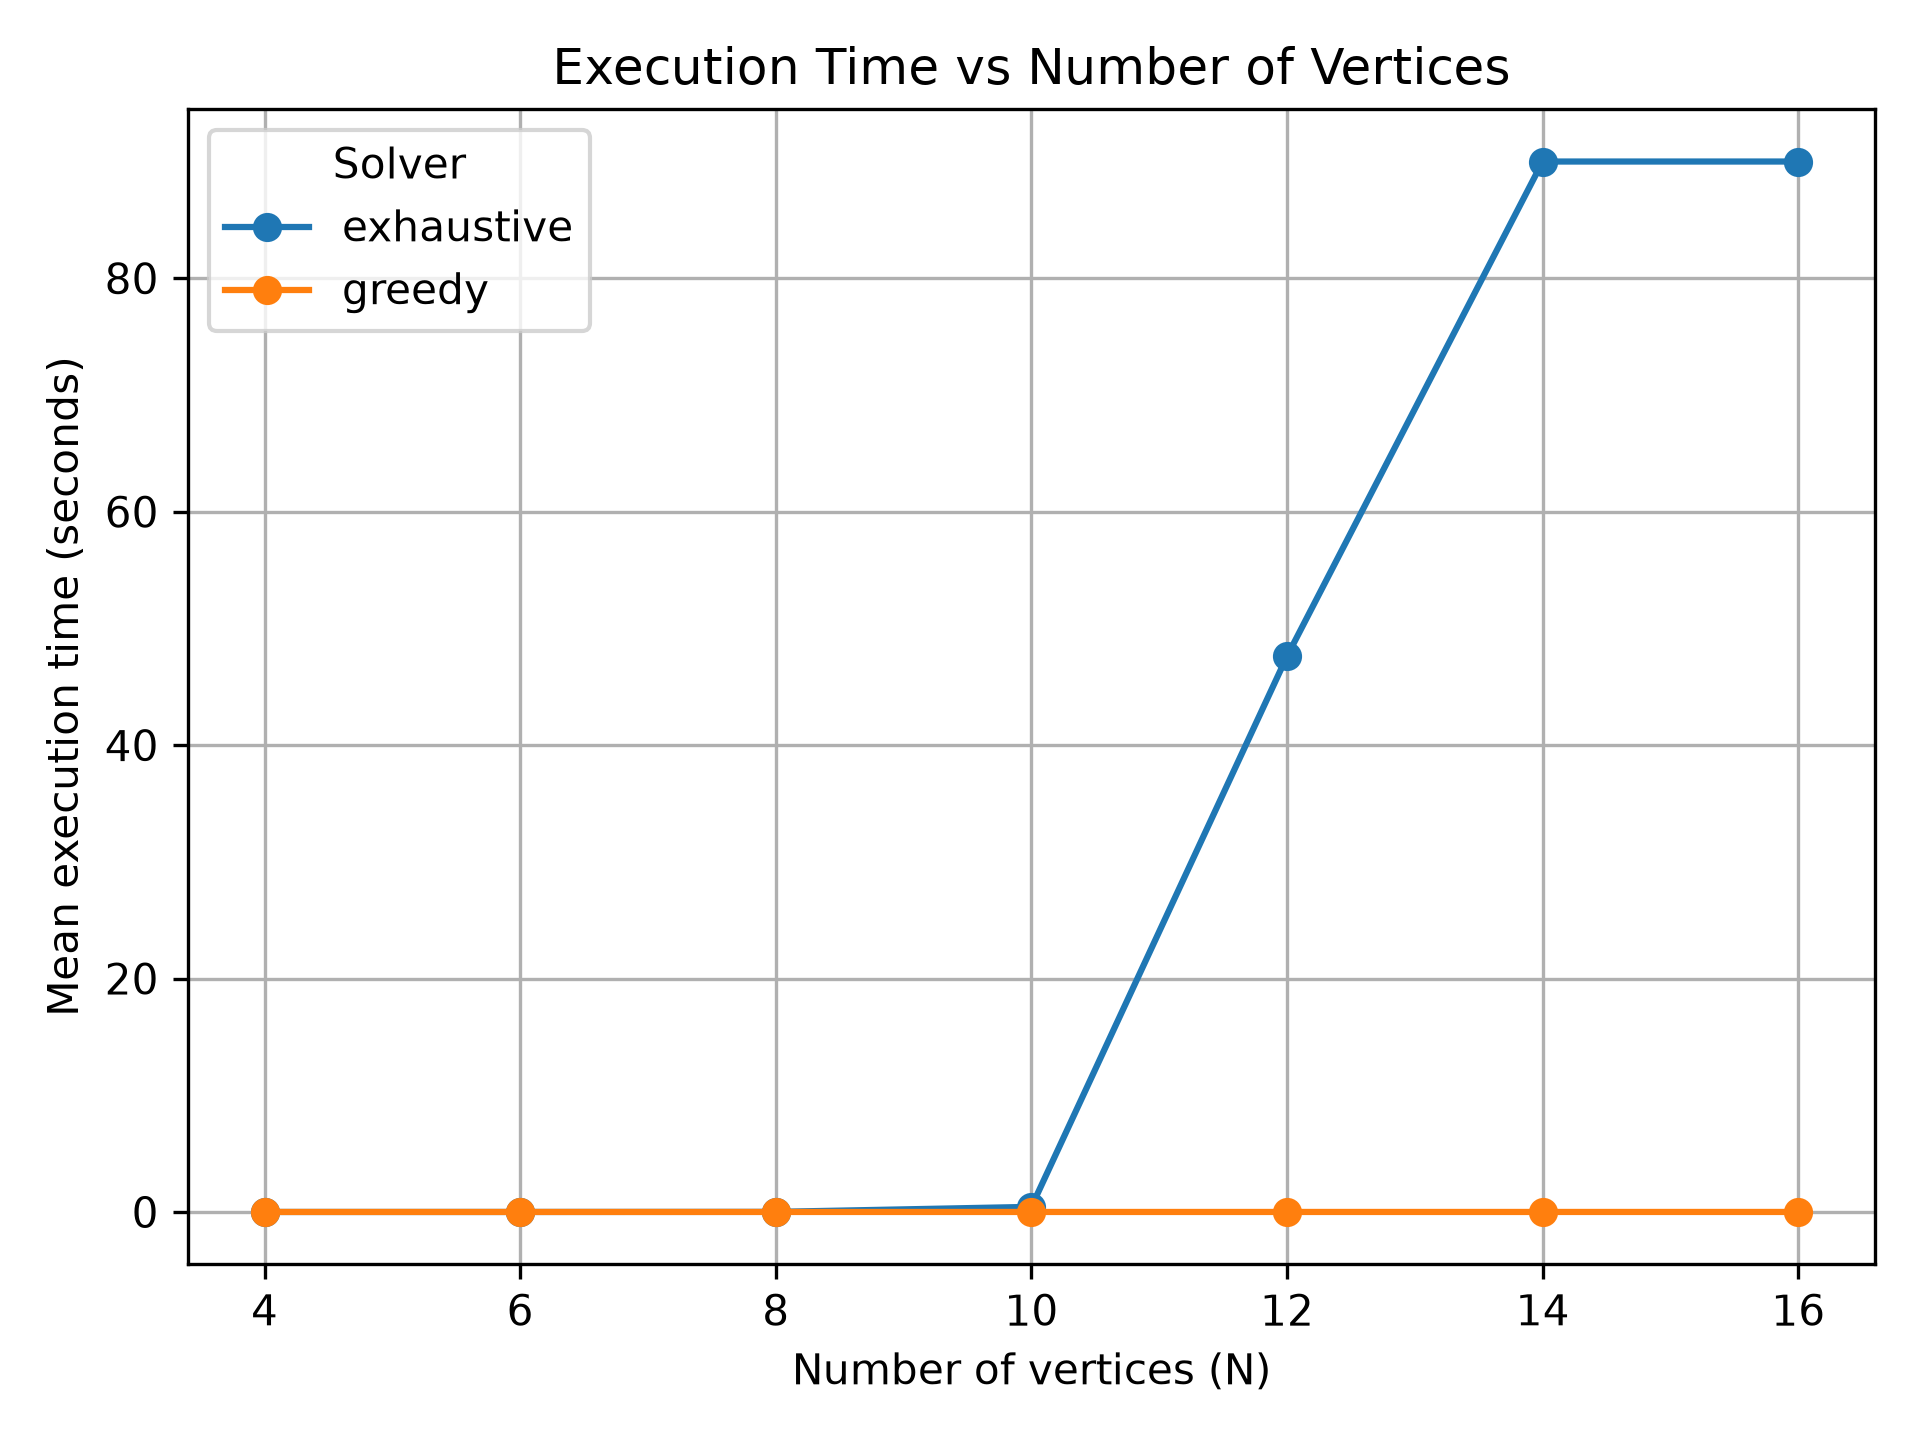
\includegraphics[width=\columnwidth]{figures/runtime_linear.png}
\caption{Execution time versus number of vertices (linear scale).}
\label{fig:runtime-linear}
\end{figure}

Figure~\ref{fig:runtime-log} presents the same comparison using
a logarithmic scale, making the differences at smaller execution
times easier to observe.

\begin{figure}[ht]
\centering
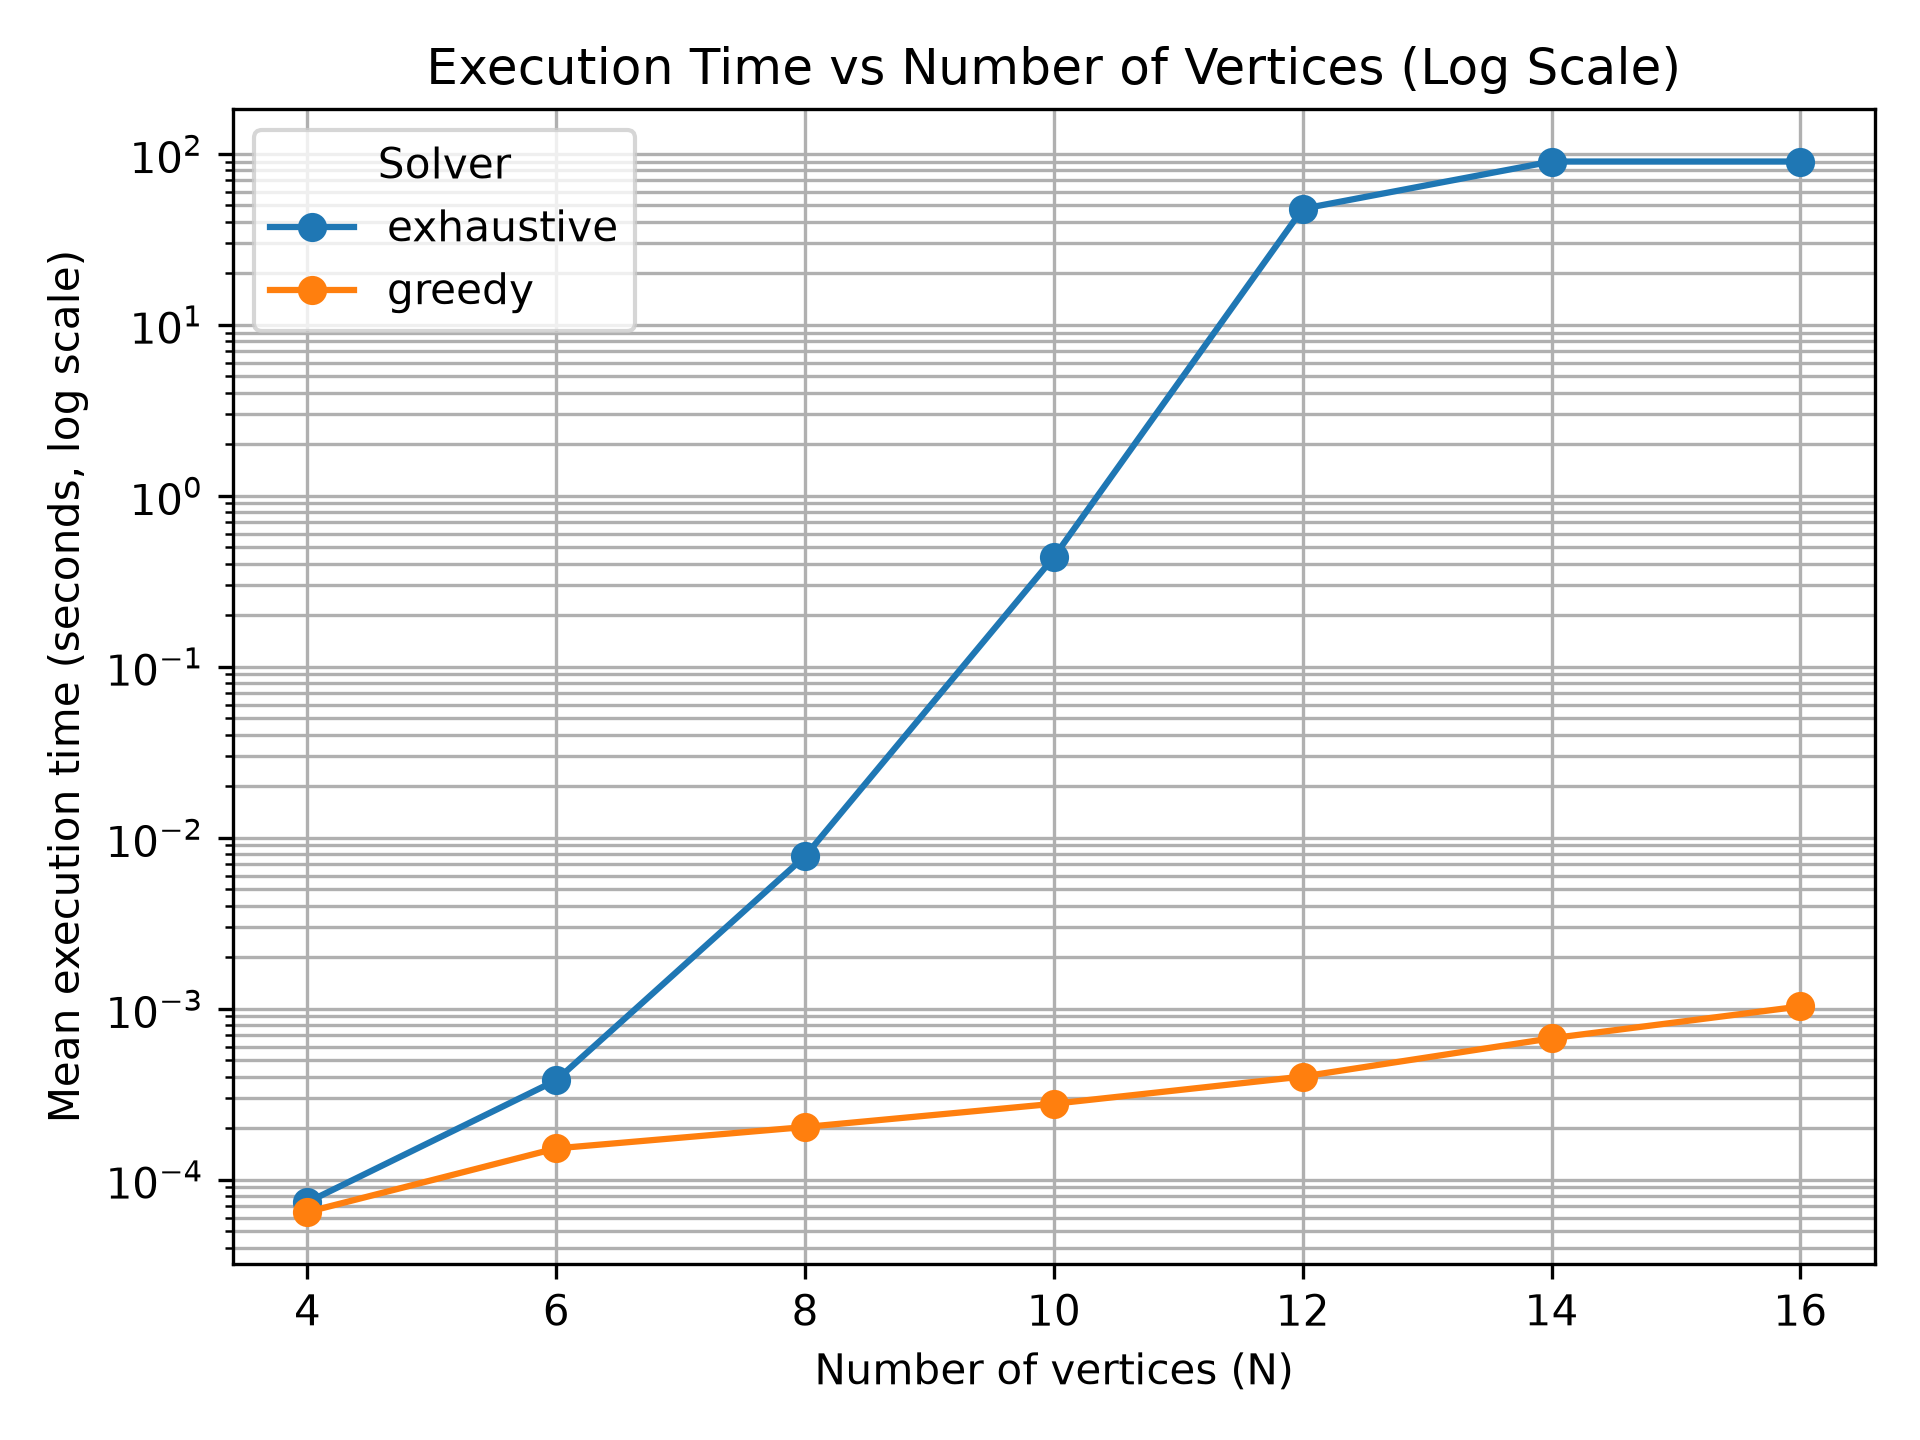
\includegraphics[width=\columnwidth]{figures/runtime_log.png}
\caption{Execution time versus number of vertices (logarithmic scale).}
\label{fig:runtime-log}
\end{figure}

The exhaustive algorithm exhibits a rapid increase in execution
time as the number of vertices grows. At 12 vertices, its mean
execution time was approximately 42.48 seconds. At 14 and 16
vertices, all four density experiments reached the 90-second
timeout.

In contrast, the greedy algorithm remained below one millisecond
on average for all tested sizes. This demonstrates its practical
speed advantage, although execution speed alone does not establish
solution quality.

\subsection{Basic Operations}

Table~\ref{tab:operations} presents the mean operation counts
for both algorithms.

\begin{table}[ht]
\centering
\caption{Mean basic operations}
\label{tab:operations}
\begin{tabular}{r r r}
\toprule
Vertices & Exhaustive & Greedy\\
\midrule
4  & 7 & 20.5\\
6  & 109 & 72.5\\
8  & 3,759 & 194\\
10 & 290,380 & 404\\
12 & 33,380,458 & 705.5\\
14 & 87,970,806 & 1,199.5\\
16 & 86,642,205 & 1,784.5\\
\bottomrule
\end{tabular}
\end{table}

Figure~\ref{fig:operations} illustrates the operation-count
comparison using a logarithmic scale.

\begin{figure}[ht]
\centering
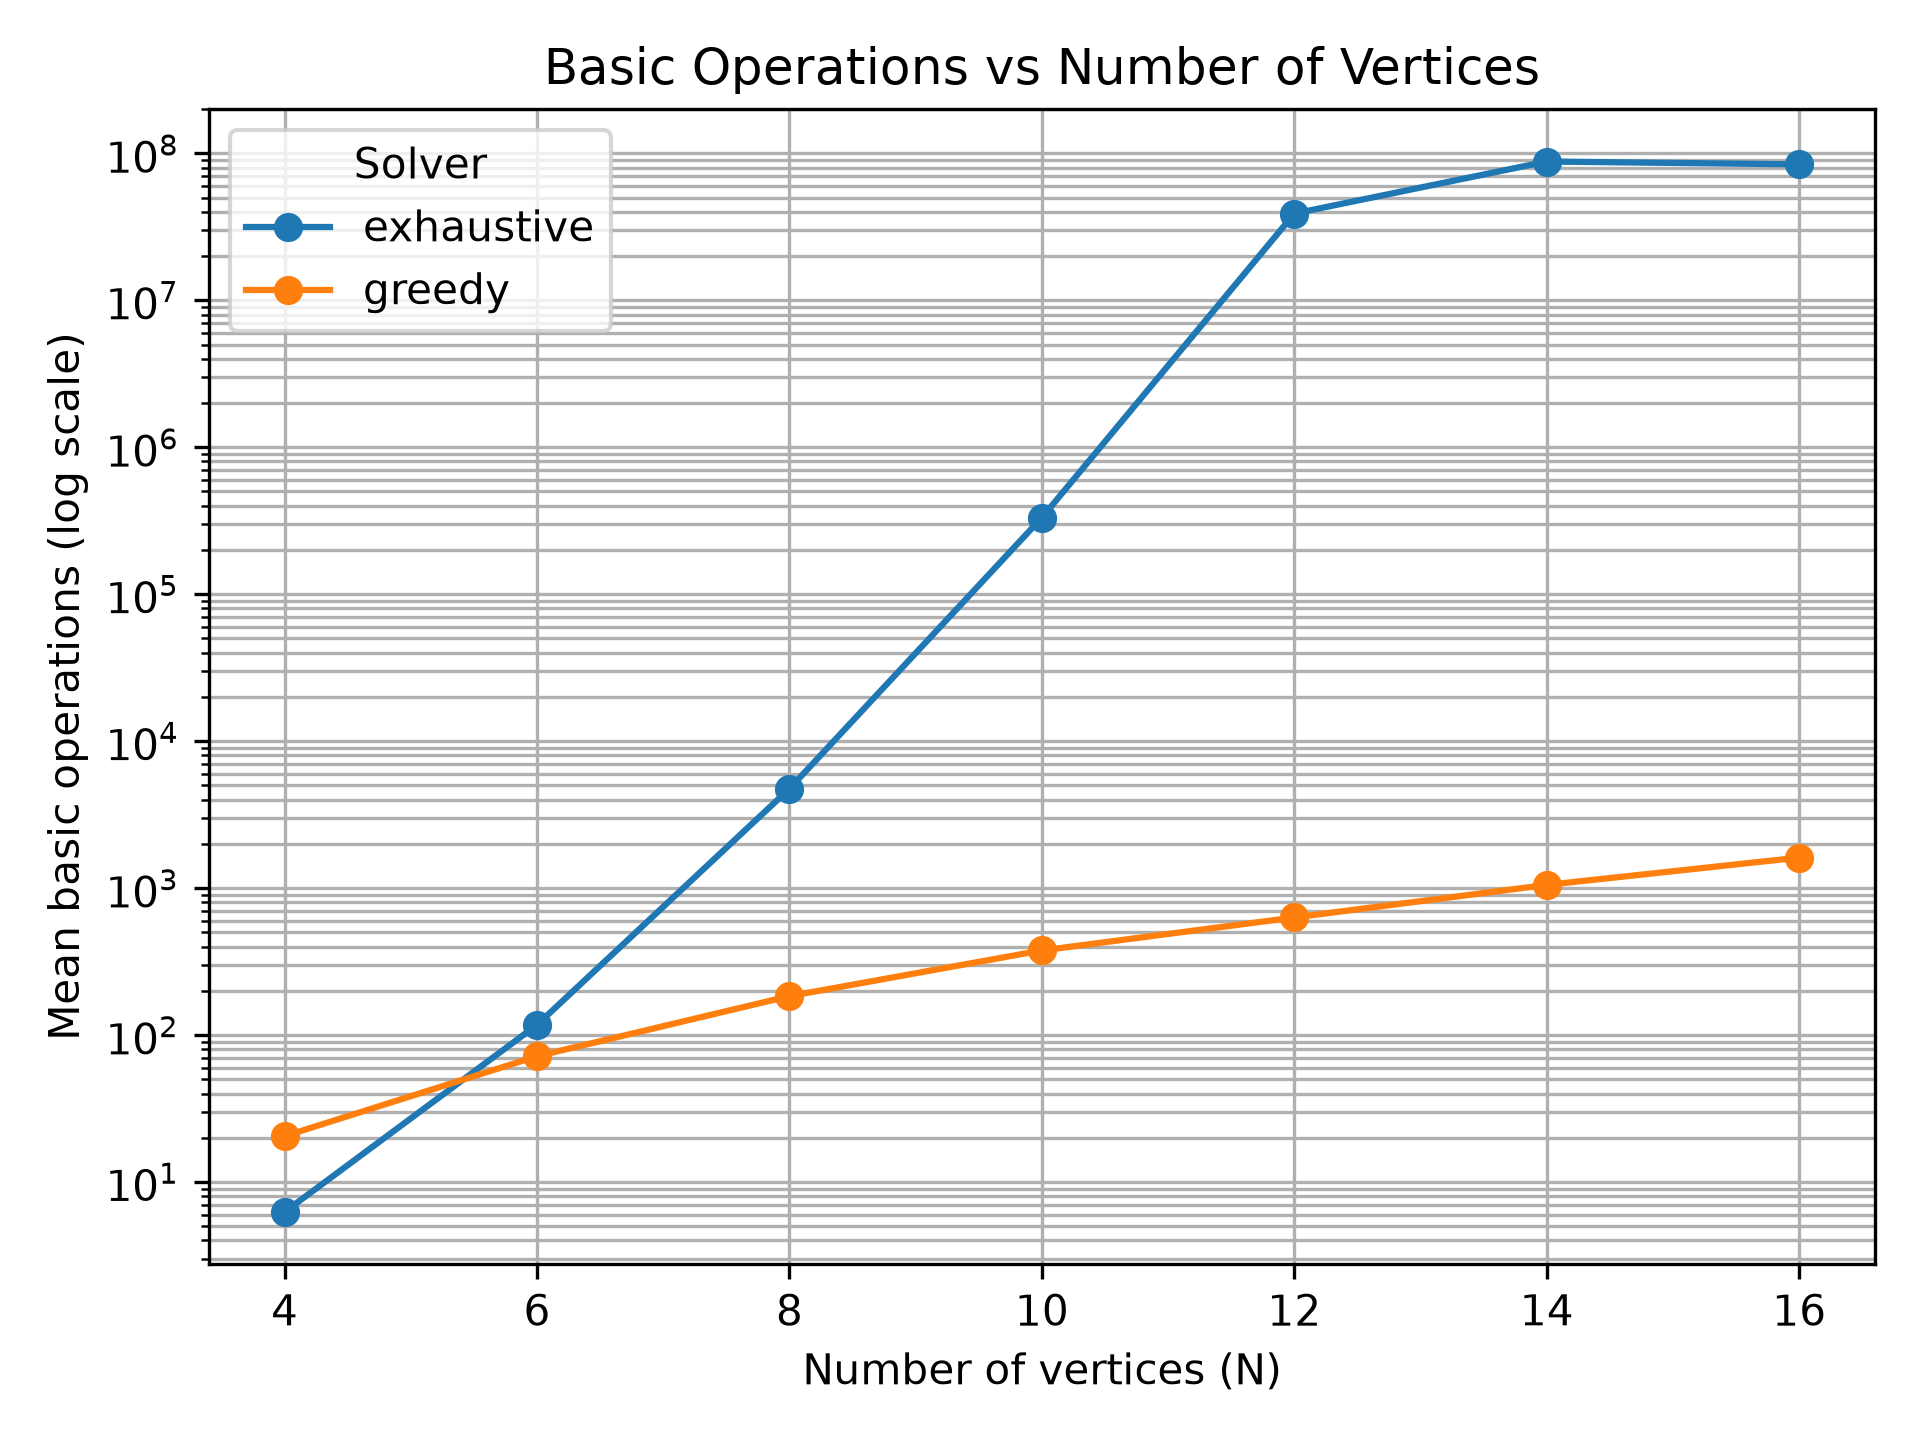
\includegraphics[width=\columnwidth]{figures/basic_operations.png}
\caption{Mean basic operations versus number of vertices.}
\label{fig:operations}
\end{figure}

The exhaustive operation count increases substantially with
graph size. Counts at 14 and 16 vertices represent partial work
before timeout, rather than completed searches. The greedy
operation count grows much more gradually.

\subsection{Optimality Gap}

Only two benchmark cases provided a valid comparison between
a completed exact solution and a feasible greedy solution.

For six vertices at 75\% density, the greedy solution matched
the optimum, producing a gap of 0\%. For ten vertices at 75\%
density, the gap was approximately 5.18\%.

Figure~\ref{fig:gap} shows the available greedy optimality-gap
measurements.

\begin{figure}[ht]
\centering
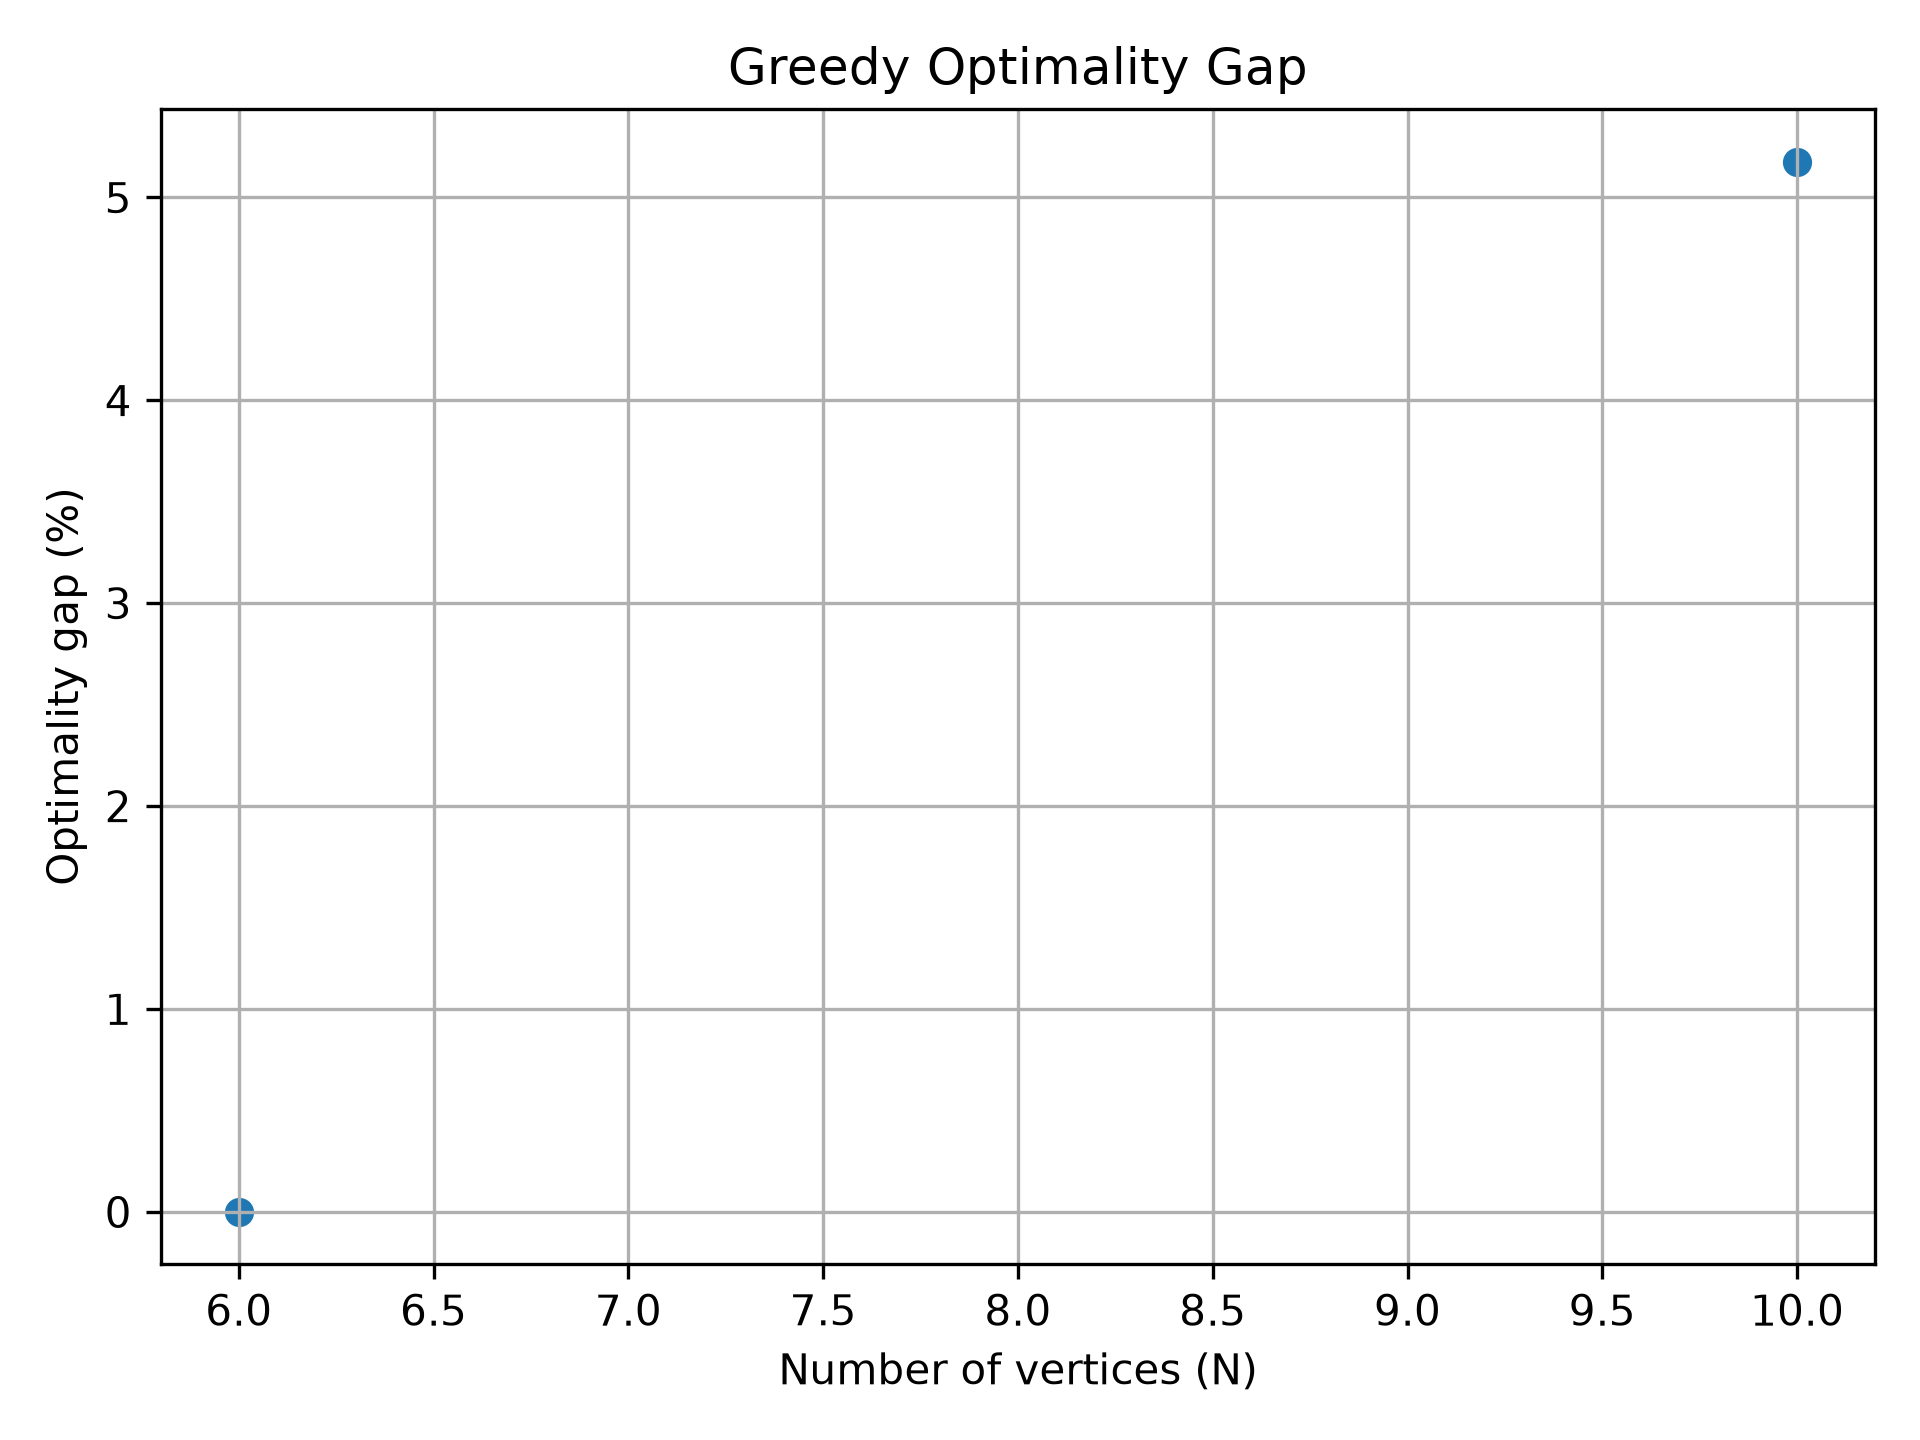
\includegraphics[width=\columnwidth]{figures/optimality_gap.png}
\caption{Optimality gap of feasible greedy solutions.}
\label{fig:gap}
\end{figure}

These two observations are insufficient to establish a general
quality guarantee. More instances with known optimal solutions
would be needed for a statistically meaningful comparison.

\subsection{Maximum Solvable Instance Size}

Under the 90-second limit, the largest tested vertex count for
which all four density experiments completed using exhaustive
search was
\[
N_{\max}=12.
\]

All exact runs at 14 and 16 vertices reached the timeout.
This empirical limit is consistent with the factorial growth
of exhaustive search. Larger instances would require more
efficient exact methods or approximation techniques.

\section{Limitations}

An important modelling limitation concerns graph density. The
synthetic instances were generated as sparse subgraphs of
Euclidean point sets. Although their edge weights are Euclidean
distances, removing edges can violate the triangle inequality
when distances between non-adjacent vertices are considered
through the remaining graph.

Therefore, these experiments evaluate Hamiltonian-cycle
optimization on sparse Euclidean-weighted graphs, rather than
the complete metric TSP under its standard assumptions.

The limited number of instances with both known exact and
greedy solutions also restricts conclusions about heuristic
solution quality. In addition, the greedy method's failure to
construct a tour should not be interpreted as proof that no
tour exists.

\section{Conclusion}

This project implemented and evaluated exhaustive search and
a deterministic multi-start nearest-neighbour heuristic for
the Traveling Salesperson Problem.

The experiments demonstrate the factorial growth of exhaustive
search and the substantially lower execution time of the greedy
approach. Under a 90-second limit, the largest tested size for
which all four density experiments completed exactly was
12 vertices.

Although the greedy method was computationally efficient, it
did not always construct a feasible tour and provided no
optimality guarantee. The small number of comparable solutions
also limits conclusions about its approximation quality.

Future work in Project 2 can investigate refined heuristics,
local search, and randomized approximation strategies to improve
solution feasibility and quality on larger instances.

\section*{Generative AI Declaration}

ChatGPT was used as an assistance tool for conceptual
explanations, debugging support, documentation, and language
and report-structure preparation. The student remains responsible
for the submitted implementation, experimental results, equations,
and interpretations. All reported experimental values originate
from the project's recorded benchmark data. The student must
review, understand, and verify the final report and code before
submission.

\bibliographystyle{e-revdetua}
\bibliography{references}

\end{document}
